
\begin{frame}
  \frametitle{Objetivo do Trabalho}
  \begin{enumerate}
    \item Transformar uma EDO em um sistema matriz-vetor
    \vspace{1cm}
    \item Resolver o sistema matriz-vetor usando métodos Iterativos
  \end{enumerate}
\end{frame}

\section{EDO para Matriz-vetor}
\begin{frame}
  \frametitle{Formulação Forte}

  Dada uma função $f : [0,1] \to \mathbb{R}$ e constantes $\alpha > 0$, $\beta \geq 0$ e $\gamma \geq 0$, queremos encontrar a função $u : [0,1] \to \mathbb{R}$ tal que:

  \vspace{0.5cm}

  \begin{center}
    $(S) = \begin{cases}
      -\alpha u_{xx}(x) + \beta u(x) + \gamma u_{x}(x) = f(x) \\
      \\
      u(0) = u(1) = 0
    \end{cases}$
  \end{center}

  \vspace{0.5cm}

  Sendo $(S)$ conhecido como a formulação forte do problema.
\end{frame}

\begin{frame}

  Visto que $-\alpha u_{xx}(x) + \beta u(x) + \gamma u_{x}(x) = f(x)$, podemos multiplicar ambos os lados por uma função $v(x)$ tal que $v(1) = v(0) = 0$ que nos ajude a eliminar a segunda derivada $u_{xx}$:

  \vspace{0.5cm}

 \[-\alpha u_{xx}(x)v(x) + \beta u(x)v(x) + \gamma u_{x}(x)v(x) = f(x)v(x)\]

 \vspace{0.5cm}

 e Integrar:

 \vspace{0.5cm}

 \[\int^{1}_{0} -\alpha u_{xx}(x)v(x) + \beta u(x)v(x) + \gamma u_{x}(x)v(x) dx = \int^{1}_{0} f(x)v(x) dx\]
\end{frame}

\begin{frame}
  Utilizando integração por partes na parcela da esquerda, temos:

  \[-\alpha \left[u_{x}(x)v(x) \bigg|^{1}_{0} - \int^{1}_{0} u_{x}(x)v_{x}(x) dx\right] + \int^{1}_{0} \beta u(x)v(x) dx + \int^{1}_{0} \gamma u_{x}(x)v(x) dx\]

  \vspace{0.3cm}

  \[-\alpha \left[- \int^{1}_{0} u_{x}(x)v_{x}(x) dx\right] + \int^{1}_{0} \beta u(x)v(x) dx + \int^{1}_{0} \gamma u_{x}(x)v(x) dx\]

  \vspace{0.3cm}

  \[\int^{1}_{0} \alpha u_{x}(x)v_{x}(x)  + \beta u(x)v(x) + \gamma  u_{x}(x)v(x) dx\]
\end{frame}

\begin{frame}[fragile]
  \frametitle{Definição da Formulação Fraca}

  Seja $H$ um espaço de funções formado por funções $u$ suficientemente suaves que satisfazem $(W)$. Seja $V$ um espaço das funções de teste, composto por funções $v$ suficientemente suaves e que satisfazem as condições de contorno $v(0) = v(1) = 0$.

  \vspace{0.3cm}

  Dados $\alpha > 0$, $\beta \geq 0$, $\gamma \geq 0$ e uma função $f : [0,1] \to \mathbb{R}$, precisamos determinar $u : [0,1] \to \mathbb{R}, u \in H$, tal que, $\forall v \in V$,

  \[(W) = \begin{cases} \displaystyle \int^{1}_{0} \alpha u_{x}(x)v_{x}(x) + \beta u(x)v(x) + \gamma u_{x}(x)v(x) dx = \int^{1}_{0} f(x)v(x) dx.\\
    \\
    u(0) = u(1) = 0
  \end{cases}\]

\end{frame}

\begin{frame}
  \frametitle{Definição do Problema Aproximado via o Método de Galerkin}

  O método de Galerkin consiste em aproximar o espaço das soluções por um espaço de dimensão finita para encontrarmos uma solução aproximada que satisfaça a formulação fraca do problema dentro de um espaço apropriado.
  \vspace{0.3cm}

  Seja $H^h$ um espaço de funções finito-dimensional composto por funções $u^h$ suficientemente suaves que satisfazem $(W)$. Analogamente, seja $V^h$ um espaço de funções finito-dimensional das funções de teste, formado por funções $v^h$ suficientemente suaves que atendem às condições de contorno $v^h(0) = v^h(1) = 0$.

  Precisamos determinar $u^h \in H^h$ tal que, $\forall v^h \in V^h$,

  \[\begin{cases} \displaystyle\int^{1}_{0} \alpha u^{h}_{x}(x)v^{h}_{x}(x) + \beta  u^{h}(x)v^{h}(x) + \gamma  u^{h}_{x}(x)v^{h}(x) dx = \int^{1}_{0} f(x)v^{h}(x) dx \\
    \\
    u(0) = u(1) = 0
  \end{cases}\]
\end{frame}

\begin{frame}
  Visto que $u^h \in H^h$, podemos tomar $u^h$ como combinação linear das funções da base de $H^h$. Seja

  \[u^h(x) = \sum_{j=1}^{m} \varphi_j(x) c_j.\]

  Logo, temos que:

  \[u_{x}^h(x) = \sum_{j=1}^{m} \varphi_{xj}(x)c_j\]

  Substituindo ambos em nossa equação:

  \vspace{0.3cm}

  \[\int_{0}^{1} \alpha \sum_{j=1}^{m} \varphi_{xj}(x) c_j v^h_x(x) + \beta \sum_{j=1}^{m} \varphi_j(x)c_j v^h(x) + \gamma \sum_{j=1}^{m} \varphi_{xj}(x)c_j v^h(x)dx\]

  \[= \int_{0}^{1} f(x) v^h(x)dx\]
\end{frame}

\begin{frame}
  \vspace{1cm}
  \[\sum_{j=1}^{m} c_j \int_{0}^{1} \alpha \varphi_{xj}(x)  v^h_x(x) + \beta \varphi_j(x) v^h(x)dx + \gamma  \varphi_{xj}(x) v^h(x)dx = \int_{0}^{1} f(x) v^h(x)dx\]
\end{frame}

\begin{frame}
  Veja que podemos tomar $v^h(x)$ como sendo qualquer função da base $V^h$.

  $v^h(x) = \varphi_i(x)$, $i \in \{1,\dots,m\}$, e $v^h_x(x) = \varphi_{xi}(x)$

  \vspace{0.3cm}

  \[\sum_{j=1}^{m} c_j \int_{0}^{1} \alpha \varphi_{xj}(x) \varphi_{xi}(x) + \beta \varphi_j(x) \varphi_i(x)dx + \gamma \varphi_{xj}(x) \varphi_i(x)dx = \int_{0}^{1} f(x) \varphi_i(x)dx\]

  \vspace{0.3cm}

  Veja que essa equação vale para $i \in \{1,\dots,m\}$. Dessa forma, podemos expressar nosso problema na forma matriz-vetor.
\end{frame}

\begin{frame}
  \[\displaystyle\sum_{j=1}^{m} c_j \int_{0}^{1}\alpha \varphi_{xj}(x) \varphi_{x1}(x) + \beta \varphi_j(x) \varphi_1(x) + \gamma \varphi_{xj}(x) \varphi_1(x)dx = \int_{0}^{1} f(x) \varphi_1(x)dx\]

  \[\vdots\]

  \[\displaystyle\sum_{j=1}^{m} c_j \int_{0}^{1} \alpha \varphi_{xj}(x) \varphi_{xi}(x)  + \beta \varphi_j(x) \varphi_i(x) + \gamma \varphi_{xj}(x) \varphi_i(x)dx = \int_{0}^{1} f(x) \varphi_i(x)dx\]

  \[\vdots\]

  \[\displaystyle\sum_{j=1}^{m} c_j \int_{0}^{1} \alpha \varphi_{xj}(x) \varphi_{xm}(x) + \beta \varphi_j(x) \varphi_m(x) + \gamma \varphi_{xj}(x) \varphi_m(x)dx = \int_{0}^{1} f(x) \varphi_m(x)dx\]
\end{frame}

\begin{frame}
\[
\begin{pmatrix}
  \mathcal{K}_{1,1} & \dots & \mathcal{K}_{1,j} & \dots & \mathcal{K}_{1,m} \\
  \vdots & \ddots & \vdots & \iddots & \vdots \\
  \mathcal{K}_{i,1} & \dots & \mathcal{K}_{i,j} & \dots & \mathcal{K}_{i,m} \\
  \vdots & \iddots & \vdots & \ddots & \vdots \\
  \mathcal{K}_{m,1} & \dots & \mathcal{K}_{m,j} & \dots & \mathcal{K}_{m,m}
\end{pmatrix}
\begin{pmatrix}
  \mathcal{C}_1 \\ \vdots \\ \mathcal{C}_i \\ \vdots \\ \mathcal{C}_m
\end{pmatrix}
=
\begin{pmatrix}
  \mathcal{F}_1 \\ \vdots \\ \mathcal{F}_i \\ \vdots \\ \mathcal{F}_m
\end{pmatrix}
\]
\end{frame}

\begin{frame}
  Para $i, j \in \{1,\dots,m\}$, tais que $i$ e $j$ correspondam aos índices da matriz, sejam:

  \begin{align*}
    \mathcal{K}_{i,j} &=\int_{0}^{1} \alpha  \varphi_{xi}(x) \varphi_{xj}(x) + \beta \varphi_i(x) \varphi_j(x) + \gamma  \varphi_i(x) \varphi_{xj}(x)dx \\
    \mathcal{F}_i &= \int_{0}^{1} f(x) \varphi_i(x) dx
  \end{align*}
\end{frame}

\begin{frame}
  \frametitle{Forma Matriz-vetor}

  Dado uma matriz $\mathcal{K}$ e um vetor $\mathcal{F}$, queremos encontrar $\mathcal{C}$ tal que:

  \[\mathcal{K}\mathcal{C} = \mathcal{F}\]

\end{frame}

\section{Tri-diagonalidade da Matriz}
\begin{frame}
  \frametitle{Escolha das Funções da Base}

  Seja $x_1, \dots, x_m$ uma discretização do intervalo $[0, 1]$ tal que $\forall i \in \{1, \dots, m\}$, $x_{i+1} - x_{i} = h$. Além disso, considere $x_0 = 0$ e $x_{m+1} = 1$ como sendo os extremos do intervalo tal que $x_{m+1} - x_m = h$ e $x_1 - x_0 = h$.

  Definiremos $\varphi_i(x)$ como:

  \[\varphi_i(x) = \begin{cases}
    \dfrac{x - x_{i-1}}{h}, &\forall x \in [x_{i-1}, x_i] \\
    \dfrac{x_{i+1} - x}{h}, &\forall x \in [x_{i}, x_{i+1}] \\
    0 , &\forall x \notin [x_{i-1}, x_{i+1}]
  \end{cases}\]

  Observe que a função base $\varphi_i(x)$ é definida como uma função linear por partes intencionalmente de forma que a sua integração e derivação sejam simples. Além disso, $\varphi_i(x)$ é projetada para ser zero fora do intervalo $[x_{i-1},x_{i+1}]$, o que significa que cada função base afeta apenas dois ou três pontos consecutivos.
\end{frame}

\begin{frame}

\[K_{i,j} = \int_{0}^{1} \alpha \varphi_{xi}(x) \varphi_{xj}(x) + \beta \varphi_i(x) \varphi_j(x) + \gamma \varphi_i(x) \varphi_{xj}(x) dx \]

  \begin{figure}[H]
    \centering
    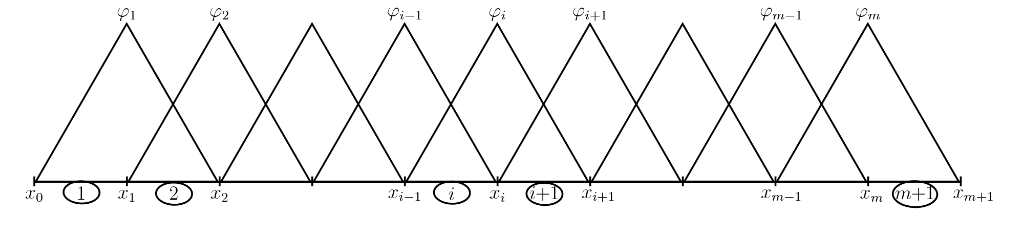
\includegraphics[width=0.9\linewidth]{phi-is.png}
    \caption{Definição das funções da base. Imagem de Bruno Alves do Carmo\cite{Bacarmo}.}
  \end{figure}
\end{frame}

\begin{frame}
  $\mathcal{K}$ é tri-diagonal!

  \vspace{1cm}

  \[\mathcal{K} =
  \begin{pmatrix}
    K_{1,1} & K_{1,2} & 0       & 0 & 0 \\
    K_{2,1} & K_{2,2} & K_{2,3} & 0 & 0 \\
    0       & K_{3,2} & K_{3,3} & \ddots & 0   \\
    0  & 0  & \ddots  & \ddots & K_{m-1,m} \\
    0  & 0  &  0      & K_{m,m-1} & K_{m,m}
  \end{pmatrix}\]
\end{frame}

\section{Métodos Iterativos}
\begin{frame}
  \begin{itemize}
    \item Contra-barra do Julia
    \item Gauss Jacobi
    \item Gauss Jacobi Tri-diagonal
    \item Gauss Jacobi Paralelo
    \item Gauss Jacobi Tri-diagonal Paralelo
    \item Gauss Seidel
    \item Gauss Seidel Tri-diagonal
  \end{itemize}
\end{frame}

\begin{frame}
  Testamos a convergência do erro para todos os métodos.
  \begin{figure}[H]
    \centering
    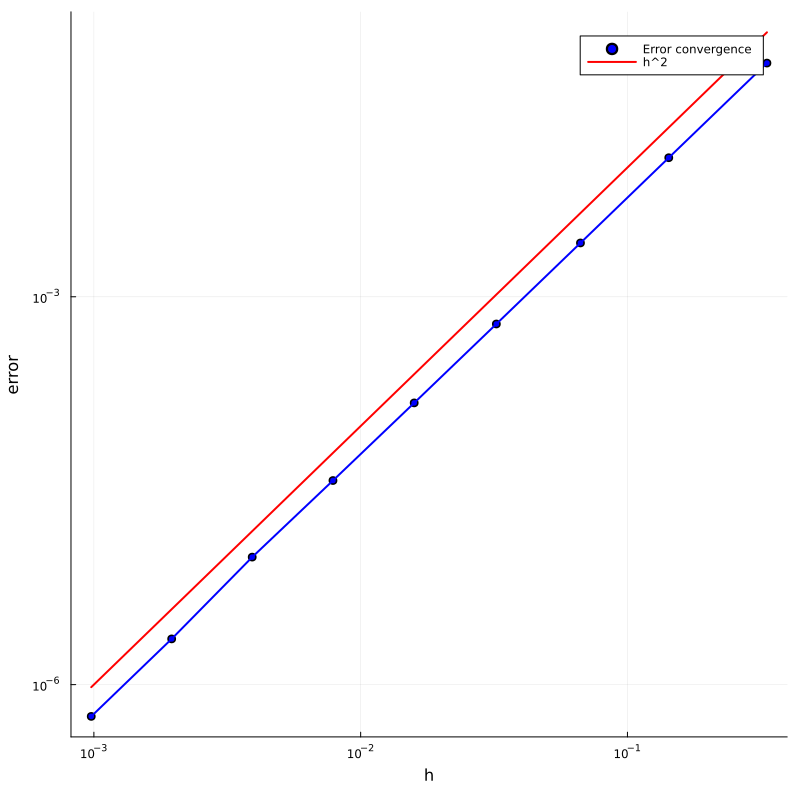
\includegraphics[width=0.55\linewidth]{errors-convergence.png}
    \caption{Convergência do Erro.}
  \end{figure}
\end{frame}

\begin{frame}
  \begin{figure}[H]
    \centering
    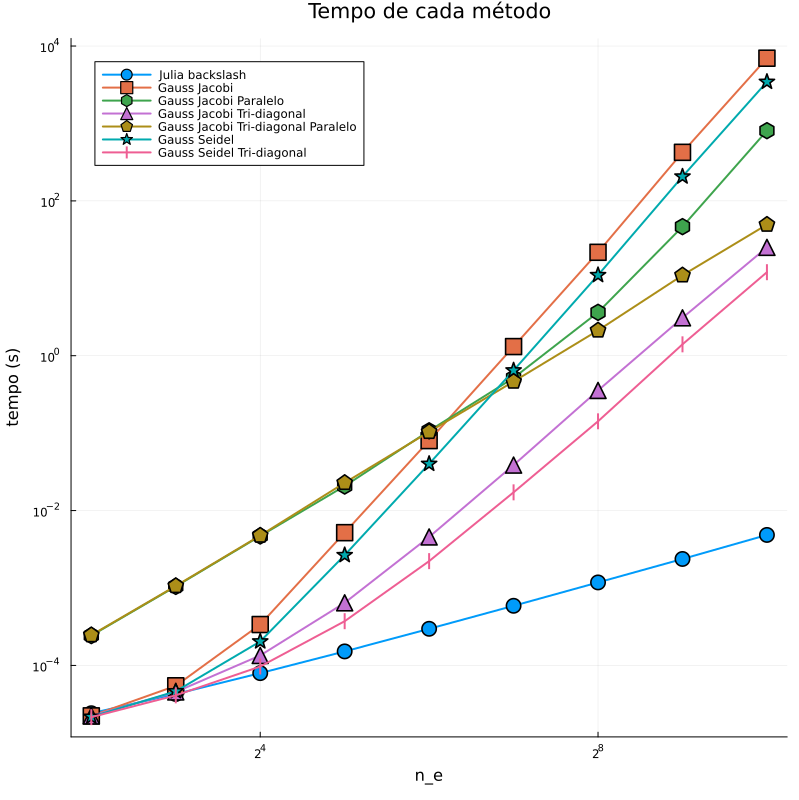
\includegraphics[width=0.6\linewidth]{compare-methods-in-solving-system-varying-ne-24-threads-2-to-10.png}
    \caption{Comparação do tempo tomado por cada método.}
  \end{figure}
\end{frame}